\documentclass{article}

\usepackage[utf8]{inputenc}
\usepackage[T1]{fontenc}
\usepackage[francais]{babel}
\usepackage{hyperref}

\hypersetup{
  unicode=false, % non-Latin characters bookmarks
  pdftoolbar=false, % show Acrobat's toolbar?
  pdfmenubar=false, % show Acrobat's menu?
  pdffitwindow=true, % page fit to window when opened
  pdfnewwindow=true, % links in new window
  pdfkeywords={polonium, P6}, % list of keywords
  colorlinks=true, % false: boxed links; true: colored links
  linkcolor=black, % color of internal links
  citecolor=green, % color of links to bibliography
  filecolor=magenta, % color of file links
  urlcolor=blue % color of external links
}

\usepackage{geometry}
\usepackage{graphicx}
\geometry{hmargin=4.0cm,vmargin=1.5cm}


\title{Solution finale projet Java\\
Projet TIA}
\author{Ronan \bsc{Abhamon}, Florian \bsc{Bigard}, Kevin \bsc{Hivert} et Nicolas \bsc{Reynaud}}
\date{2014}

\begin{document}

\maketitle

\newpage

\renewcommand{\contentsname}{Sommaire}
\tableofcontents
\newpage


\section{Introduction}
Nous avions comme idée première de faire un site à la YouTube. Après réflexion et suite aux 6 projets à réaliser en moins d'un mois grâce à une administration particulièrement performante, nous nous sommes mis d'accord de ne mettre que des liens de vidéos (permettant de les héberger sous DailyMotion, Youtube ou autre...).

\paragraph{}Dans ce rapport, nous étudierons la conception du projet (client lourd, client léger). Cette partie comprendra différents schémas et explications. Nous ferons ensuite une description des fonctionnalités que nous avons intégrées à notre projet. Pour réaliser ces fonctionnalités, nous avons dû utiliser différentes technologies dont nous expliquerons l'intégration dans la partie suivante. Nous parlerons ensuite des différents codes inspirés d'Internet qui nous ont aidés sur certaines parties. Nous finirons par une estimation du temps de chaque partie, puis à une conclusion qui comprendra un bilan critique et autres conneries demandées dans le sujet.



\section{Description générale de l'application}

Le but de notre projet est de proposer une interface Web permettant l'échange de vidéos au sein d'une communauté.
Le système part d'un concept simple : l'Internet regorge de vidéos en tout genre, pourquoi ne pas centraliser celles dignes d'intérêt ?

\paragraph{}
Cette communauté étant un ensemble de membres, nous avons donc créé un espace pour chaque membre. Qui dit espace dit aussi : 
\begin{itemize}
\item compte
\item inscription
\item connexion
\end{itemize}

Ces membres peuvent partager des vidéos de plateformes de médias comme par exemple YouTube
(et non pas les télécharger de leurs ordinateurs) sur notre application.
Le fait de partager n'est pas suffisant, ils peuvent aussi émettre une critique sur ces médias : un système de votes est donc important. Pour renforcer ce système, la mise en place de commentaires nous a semblé aussi très utile. 

\paragraph{}
Ces membres doivent donc interagir sur notre application, celle-ci est constituée de 2 environnements :
\begin{itemize}
	\item Un site internet léger pour accéder aux vidéos, commentaires et autres informations.
	\item Un client lourd, soit un programme permettant d'accéder aux mêmes données que le site internet lui-même.
\end{itemize}

\paragraph{} 
Concernant les vidéos, elles peuvent être intégrées dans des playlists. Elles peuvent donc être 
échangées entre les membres de cette communauté. Les vidéos n'étant rien d'autre que des urls dans notre base de données, une simple recherche de mots clefs peut mener à un ensemble de vidéos.
Une fonction recherche est donc indispensable. 
Enfin les utilisateurs ont la possibilité de trier ces vidéos par date, nombre de votes ou nom.

\paragraph{}
Enfin, un tchat permet aux membres de communiquer entre eux. S'ils sont tous deux connectés, ils communiquent directement à l'aide de sockets. Sinon ils communiquent grâce au serveur qui stocke les messages en attendant que l'autre personne se connecte et lise ses propres messages.



\section{Conception}

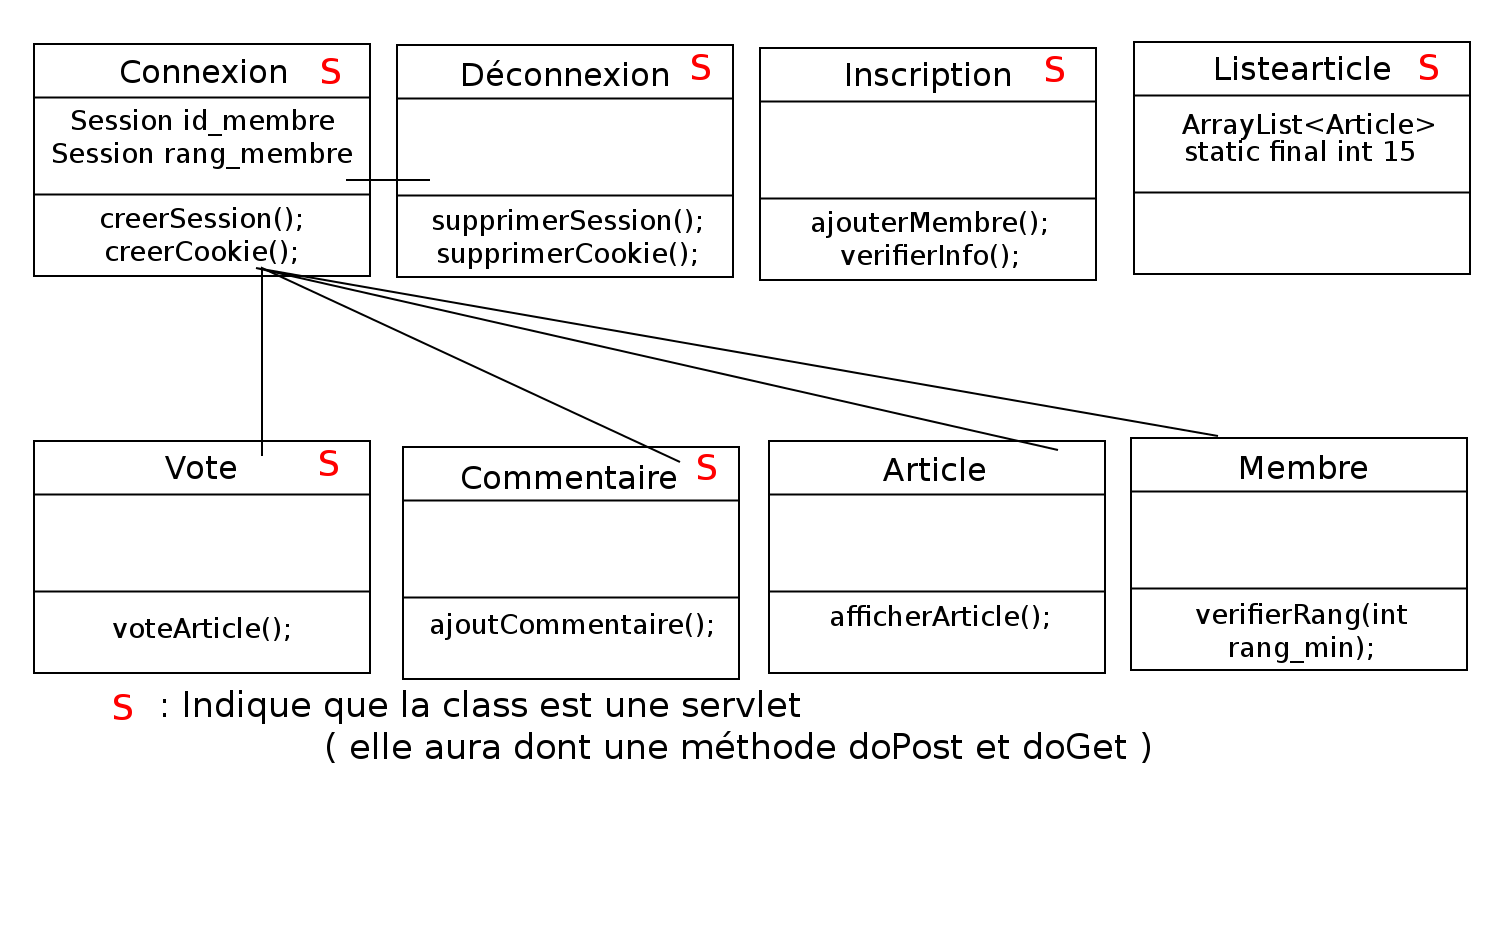
\includegraphics[scale=0.4, angle=90]{UML.png}


\section{Plan du site}

\subsection{Pages principales}
\begin{center}
Design des pages principales
\end{center}
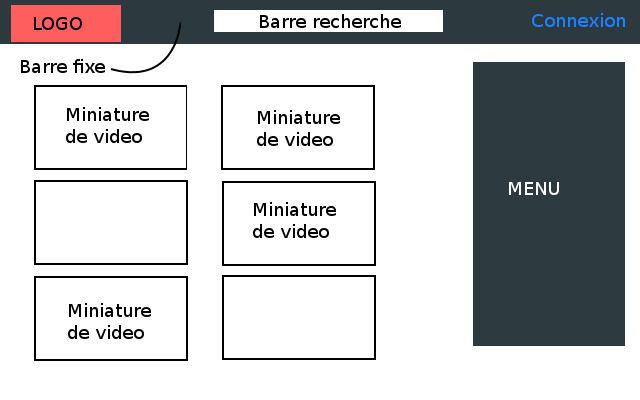
\includegraphics[scale=0.7]{design.png}


\subsubsection{Accueil}
La page d'accueil contient les miniatures des vidéos qui ont déjà été postées. Celles ci sont triées par date de publication de la plus récente à la plus ancienne.
Il s'agit de la première page visible sur le site à l'arrivée d'un visiteur.

\subsubsection{Top - Flop}
Les pages Top et Flop ont pratiquement la même fonction que la page d'accueil, cependant la page Top trie les vidéos par nombre de votes décroissants [ des plus appréciées aux moins appréciées ]. La page Flop quant à elle trie dans le nombre croissant de votes [ Des moins appréciées aux plus appréciées ].

\subsection{Pages associées à une vidéo}
\begin{center}
Design des pages d'affichage de vidéos :
\end{center}
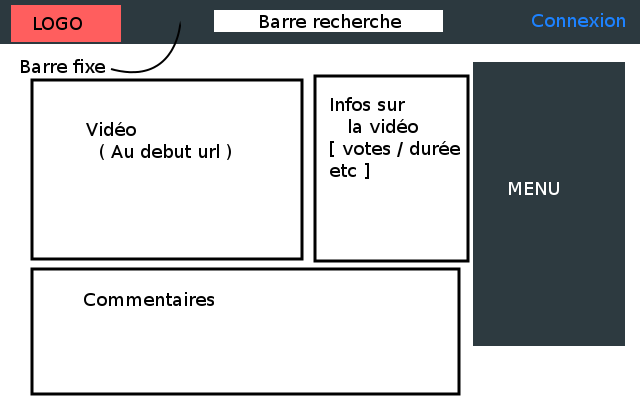
\includegraphics[scale=0.7]{pages.png}
Sur cette page, un membre peut, mettre en favoris la vidéo, voter pour cette vidéo et la commenter.\\
\subsubsection{Visualisation d'une vidéo}

\subsubsection{Random}
La page random donne une vidéo de façon aléatoire parmi toutes celles disponibles sur le site.


\subsection{Pages secondaires - Formulaires}
\begin{center}
Design des pages secondaires :
\end{center}
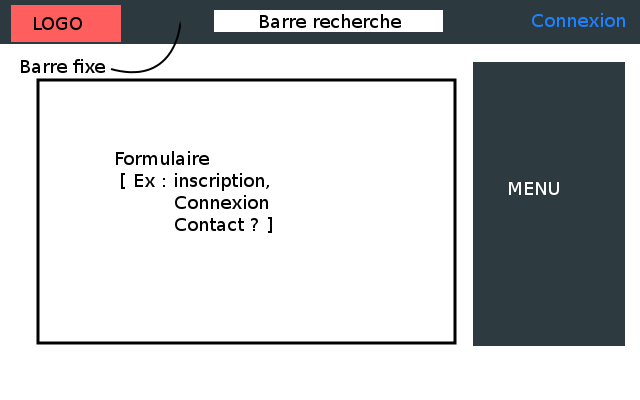
\includegraphics[scale=0.7]{formulaires.png}

\subsubsection{Inscription}
Cette page permet à un visiteur de s'inscrire pour qu'il devienne membre de la communauté.

\subsubsection{Connexion}
La page connexion permet aux membres du site de se connecter en passant leur statut de visiteur à membre.

\subsubsection{Déconnexion}
La page déconnexion a pour but de déconnecter une personne si elle est connectée.

\subsubsection{Poster article}
Cette page permet simplement aux membres de poster un article.

\section{Description des fonctionnalités}
Notre projet propose donc un certain nombre de fonctionnalités, ces dernières étant identiques sur chaque support comme il l'était stipulé dans l'énoncé du projet.

\paragraph{}Les utilisateurs étant enregistrés dans une base de données la première fonctionnalité est bien entendu l'inscription, la connexion et la déconnexion d'un membre. Ainsi les vidéos, commentaires etc... peuvent être attribués à un membre précis de la communauté.

\paragraph{}Les membres ainsi que les visiteurs peuvent chercher et visionner par la suite des vidéos, les recherches se font par rapport aux titres des vidéos mais 4 types de tri sont possibles :
	\begin{itemize}
	\item Popularité décroissante : Les vidéos ayant le plus fort indice de popularité sont donc affichées en haut de la liste.
	\item Popularité croissante : Ici ce sont donc les vidéos ayant le plus faible indice de popularité qui sont affichées en premier.
	\item Date décroissante : Les vidéos sont donc affichées de la plus récente à la plus ancienne, c'est un bon moyen pour voir les nouveautés.
	\item Date croissante : Les vidéos sont triées de la plus ancienne à la plus récente, un tri pour les plus nostalgiques donc.
	\end{itemize}
\subparagraph{}Le visionnage d'une vidéo affiche le titre de la vidéo, la popularité, la description ainsi que la liste des commentaires. Le client léger affiche la vidéo si le lien mène bien vers une vidéo valide, le client lourd lui, permet d'accéder à la vidéo sur internet grâce à son lien.

\paragraph{}Les membres connectés ont, comme nous l'avons vu, la possibilité de regarder les vidéos, tout comme les visiteurs non enregistrés mais contrairement à ces derniers les membres ont la possibilité de pouvoir voter, commenter et ajouter une vidéo à leurs favoris.
\subparagraph{}Les votes nous permettent par la suite de créer un classement par popularité, un vote pouvant être positif ou négatif. Chaque vote ajoute ou enlève 1 point à la popularité de la vidéo.
\subparagraph{}Les commentaires permettent aux membres d'exprimer leurs avis, de discuter et d'échanger autour d'une vidéo.
\subparagraph{}Les membres peuvent également ajouter une vidéo à leur playlist personnel, nous décrirons ce point juste après.

\paragraph{}Les membres possèdent donc chacun une playlist, à laquelle ils peuvent ajouter des vidéos afin de les conserver et les retrouver plus facilement.
\subparagraph{}Cette playlist peut \^etre exportée sous format XML afin d'\^etre partagée avec les autres membres de la communauté, au tout autre but que pourrait trouver l'utilisateur.

\paragraph{}Les membres ont évidemment la possibilité d'ajouter des vidéos et ainsi les partager avec le reste de la communauté (pas celle de l'anneau). Lorsqu'un membre ajoute une vidéo on lui demande le lien vers une vidéo (Youtube ou autre). Il lui est également demandé un lien vers une miniature à afficher, ainsi qu'un titre et une description de la vidéo.
\subparagraph{}Nous voulions ajouter la possibilité de modifier les vidéos, cependant le manque de temps aura eu raison de cette fonctionnalité. Une autre fonction qui n'a pas pu voir le jour est un système de rang par lequel des administrateurs et des modérateurs auraient pu modifier voir supprimer certaines vidéos si le contenu n'était pas convenable.


\section{Technologies mises en oeuvre}

\subsection{Client lourd}

\subsubsection{Tchat}
Pour la réalisation du Tchat, nous avons dû nous servir des sockets couplés à des threads, comme lors du TP2 (serveur convertisseur).

\subsubsection{Swing}
Swing a permis de construire une interface fonctionnelle. Cependant Swing contraint à utiliser des Components pouvant vite devenir incontrôlables d'où l'utilisation d'une classe \href{http://tips4java.wordpress.com/2008/11/06/wrap-layout/}{http://WrapLayout}
pour fixer facilement certains éléments sensibles. Nous pensons notamment aux miniatures des vidéos.

\subsubsection{Singleton}
Nous avons aussi créé une classe singleton nous permettant de stocker les informations du membre qui utilise le client lourd. Nous pouvons donc ensuite récupérer simplement les différentes informations (id, ip, pseudo...).

\subsubsection{Template}
La partie Swing du projet dispose de plusieurs classes comme les aperçus des vidéos découlant de templates (Patron de méthode). Cela permet de définir un comportement global de classe mais permet aussi de définir des interactions différentes pour les classes héritantes.

\subsection{Client léger}

\subsubsection{Jsp}
Les jsp font partie intégrante de cette partie, j'ai également pu également utiliser les inclusions que celle ci fournissait afin de bien séparer chaque partie du projet.

\subsubsection{Servlet}
J'ai pu utiliser les Servlets, lequel m'on permis de générer les XML afin de passer les données au client Lourd, en fonction des données qui m'était envoyé par le client lourd.\\

\subsubsection{SQL}
Bien entendu, j'ai du utiliser le SQL afin de faire mes requetes sur la base de données. Ce qui implique également d'utiliser les connexion depuis Java, notamment a l'aide de la librairie externe : "jdbc".\\

\section{Codes inspirés d'Internet}
\subsection{Partie réseau}
Pour la réalisation de l'API, nous avions besoin de communiquer avec le serveur via des requêtes HTTP (POST et GET). Cette partie fut un peu plus délicate, il nous a fallu aller chercher sur StackOverflow une aide pour la réalisation de ce type de requête. Nous n'irons pas vous cacher notre étonnement lorsque nous nous sommes rendus compte que chacune des méthodes faisait dans les 100 lignes. 


\section{Estimation du temps}
\subsection{Client léger}
Le temps passé sur le client léger est très conséquent pour ma part, ( Reynaud Nicolas) , ayant travaillé seul sur ce dernier , j'y ai passé mes nuits et mes week-end, de même que pour le design et la gestion de la Bdd.
Pour le tout, je pense être à plus de 60 heures de boulot. [ Par exemple travail du week end de 3 jours que nous avons eu :  19 au 21;
le 19 : 18h00 - 4h30;le 20 : 10h00 - 22h00; le 21 : 10h00 : 0h00 ].\\
Ainsi le temps consacré est vraiment très conséquent.\\
Cependant j'ai pu apprécier la modularité, si un changement m'était demandé, par exemple sur une requête SQL, je n'avais qu'une petite modification à faire.

\subsection{Client lourd}
Le temps consacré au client lourd est conséquent, le temps de mise en place de l'interface graphique ainsi que des parsers XML doit bien atteindre les 40h.
C'est assez important mais il existe une explication : Faire une interface accessible sans être repoussante, ainsi que positionner
correctement les éléments, ce n'est pas simple. D'autant plus de le faire proprement.
 
\subsection{Tchat}
Nous avons dû compter la bagatelle d'environ 30 heures pour réaliser la partie conception et mécanique du Tchat. Nous comptons dans ce nombre d'heures l'intégration à l'interface du client lourd.
La conception fut assez difficile à mettre en oeuvre, car il nous a fallu manipuler des Thread couplés avec des Sockets ce qui n'était pas évident. De plus la création de tests fut encore une fois difficile dans le sens où nous ne pouvions lancer deux fois le logiciel sur un seul ordinateur étant donné que celui-ci écoutait sur un port précis. 

\section{Ressources utilisées}

Comme indiqué dans la partie Swing, une unique ressource a été utilisée telle quelle pour l'interface : 
\href{http://tips4java.wordpress.com/2008/11/06/wrap-layout/}{http://WrapLayout}

La majorité du temps StackOverflow a sauvé le projet.
 
\section{Conclusion}

Les interfaces et menus prévus ont été effectués dans les temps. Cependant Swing est assez limité pour concevoir rapidement une interface complexe. (A côté il existe d'un côté GTK mais le temps de dev explose littéralement avec cette lib, et d'un autre Qt où il est possible de faire des fenêtres en utilisant du CSS.)

Pour conclure, nous avons du simplifier certaines idées que nous avions afin de pouvoir tenir les délais de plus nous pensons sincèrement que la JAVA n'est pas un langage adapté pour un projet WEB. Il existe des technos plus récentes et plus puissantes qui nous auraient permis de faire plus dans le même temps imparti, le projet en aurait été que plus intéressant et plus agréable, mais puisqu'il faut bien se plier aux règles nous avons fait de notre mieux pour fournir une applications décente et pas trop désagréable à l'oeil. 

\end{document}